\section{Reproducability: Did the Heidelberg-Moscow experiment measure neutrinoless double beta decays?}
\begin{frame}{No - The GERmanium Detector Array (GERDA)}
	\begin{columns}
		\begin{column}{.7\textwidth}
			\begin{itemize}
				\item Also located at Gran Sasso (With all HdM detectors)
				\item Fully submerged in liquid argon (cooling and shielding)
				\item Surrounded by \SI{3}{\meter} of water (with installed PMTs for $\mu$-detection)
				\item For the first time in $0\nu\beta\beta$ research: blinded analysis
				\item Run I: 2011--2013 (\SI{215}{\mole\year}) Run II: 2015-2017 (\SI{470}{\mole\year})
			\end{itemize}
		\end{column}
		\begin{column}{.29\textwidth}
			\begin{figure}
				\centering
				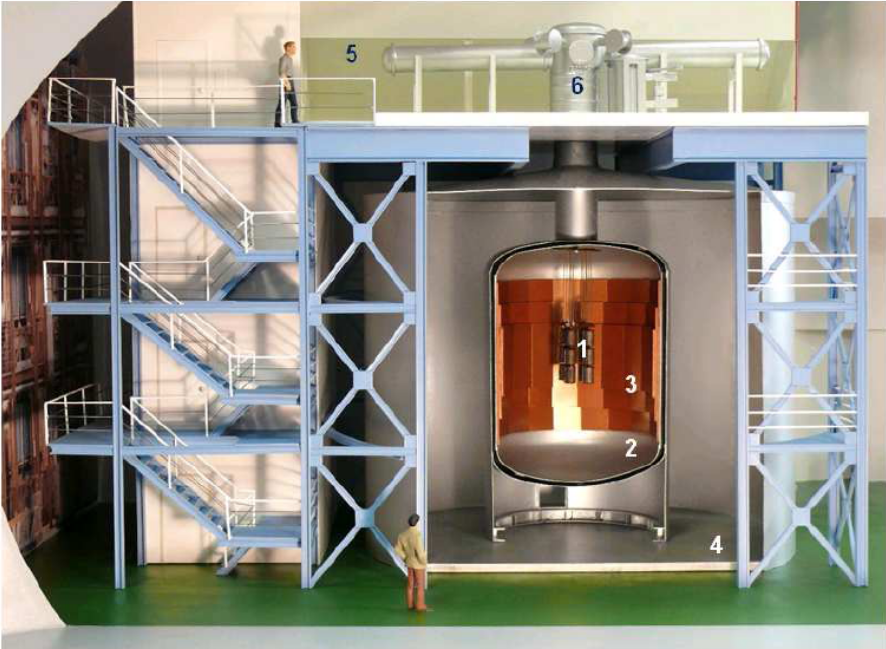
\includegraphics[trim=230 0 0 0,clip,width=\textwidth]{media/GERDA.png}
				\caption*{\hspace{-25em}GERDA (not to scale) \footnotemark[1]}
			\end{figure}
		\end{column}
	\end{columns}
	\footnotetext[1]{\fullcite{GERDAsetup}}
\end{frame}
\begin{frame}
	\frametitle{No - The GERmanium Detector Array (GERDA)}
	\begin{itemize}
		\item Currently the most sensitive experiments are ${}^{136}\symup{Xe}$, but due to the different nuclear matrix element,
			it is hard to compare them to HdM
		\item GERDA concluted at end of Run I: \enquote{The Gerda data show no indication of a peak at $Q_{\beta\beta}$, i.e. the claim for the observation of 0νββ decay in ${}^{76}Ge$ is not supported.}
		\item With the best fit value from HdM\footnote{\fullcite{Klapdor-Kleingrothaus:2001}} \num{5.9+-1.4} are expected \num{0} are detected 
	\end{itemize}
\end{frame}
